\documentclass{beamer}
\usepackage{graphicx}
\usepackage[T1]{fontenc}

\title{Kanto: FPGA Audio Player and Visualizer}
\author{
  Kavita Jain-Cocks
  \and
  Zhehao Mao
  \and
  Amrita Mazumdar
  \and
  Darien Nurse
  \and
  Jonathan Yu}

\begin{document}
\begin{frame}
	\titlepage
\end{frame}

\begin{frame}{Project Overview}
	\begin{itemize}
		\item Objective: Design and implement an audio player with frequency visuzalization.
		\item Hardware: Handles audio output and frequency visualization
		\item Software: Handles user interation and system initialization
	\end{itemize}
\end{frame}

\begin{frame}{High-Level Overview}
	\centering
	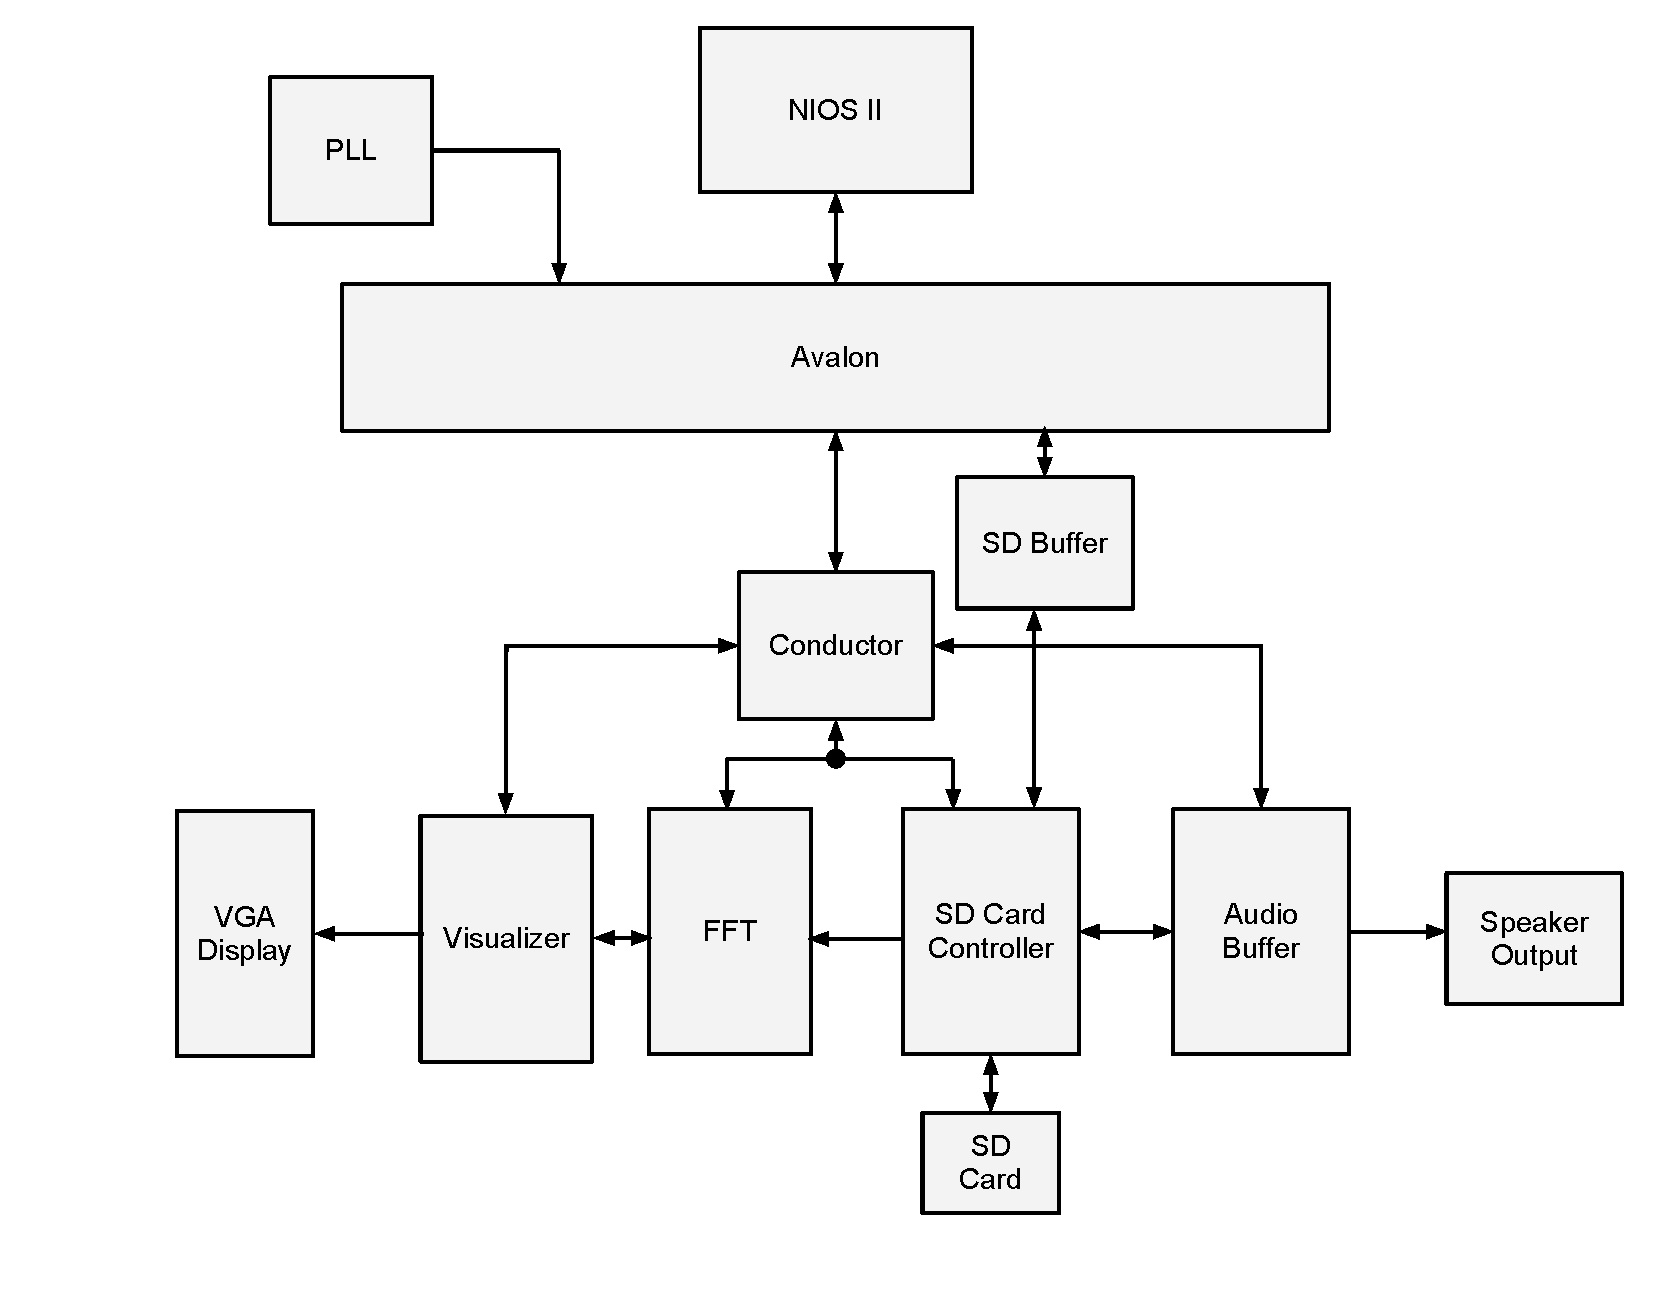
\includegraphics[width=4in]{top_level}
\end{frame}

\begin{frame}{SD Controller}
	\centering
	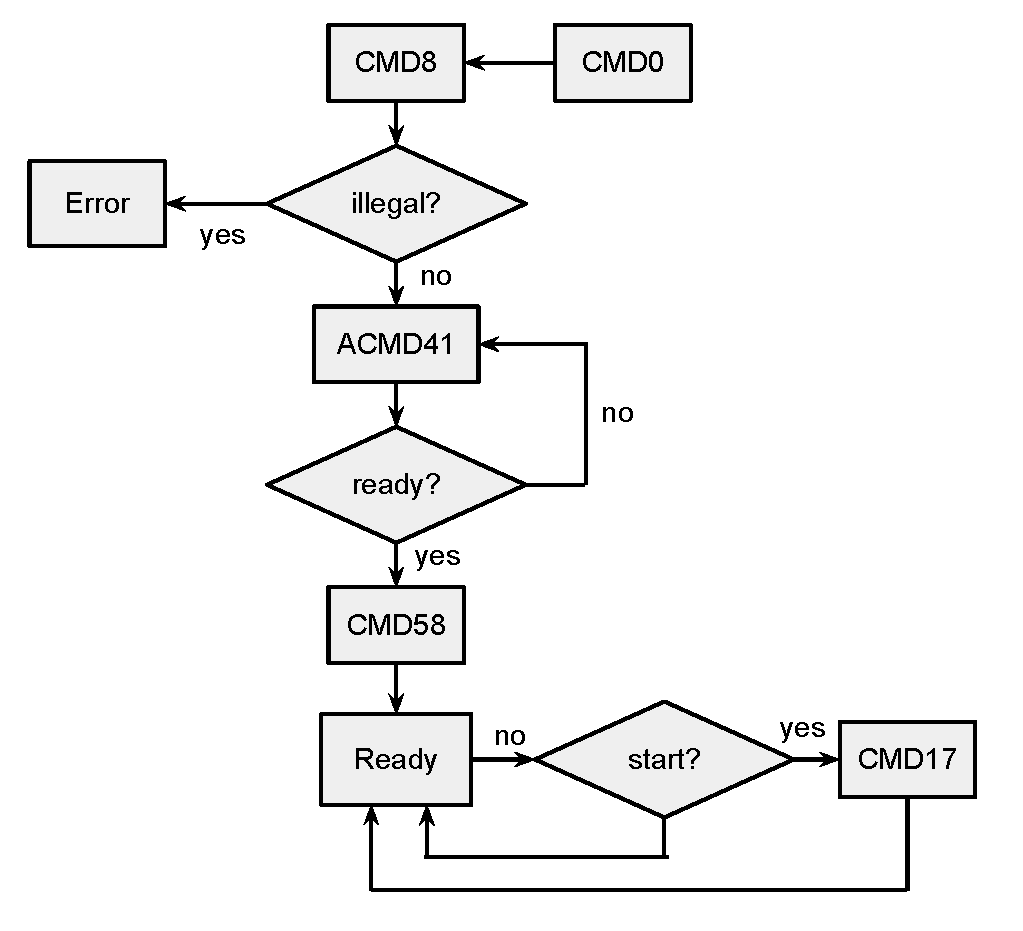
\includegraphics[height=3in]{sd-controller}
\end{frame}

\begin{frame}{Audio Buffer}
	\centering
	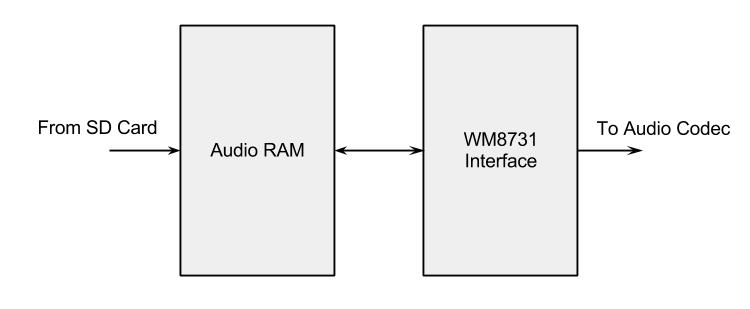
\includegraphics[width=4in]{audio-buffer}
\end{frame}

\begin{frame}{FFT Top-Level}
	\centering
	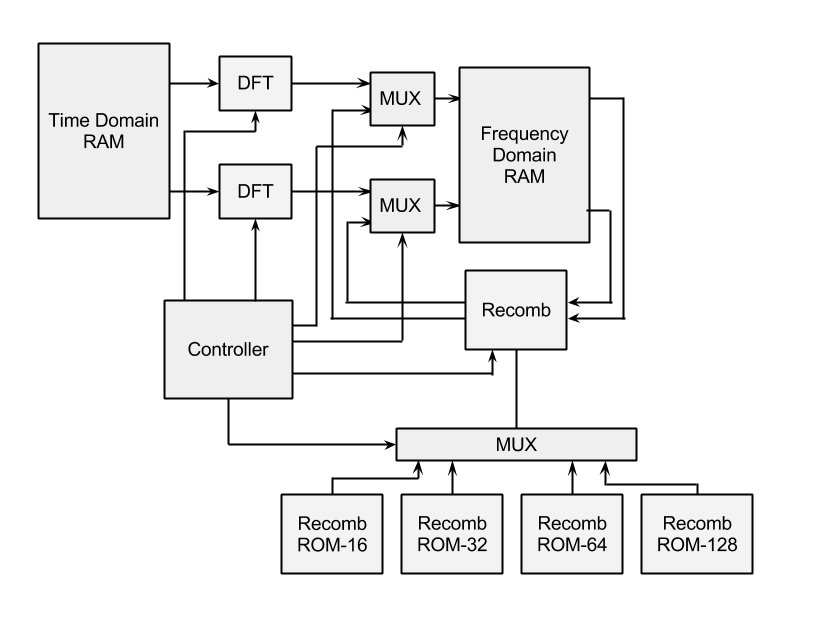
\includegraphics[width=4in]{fft-top}
\end{frame}

\begin{frame}{DFT Unit}
	\centering
	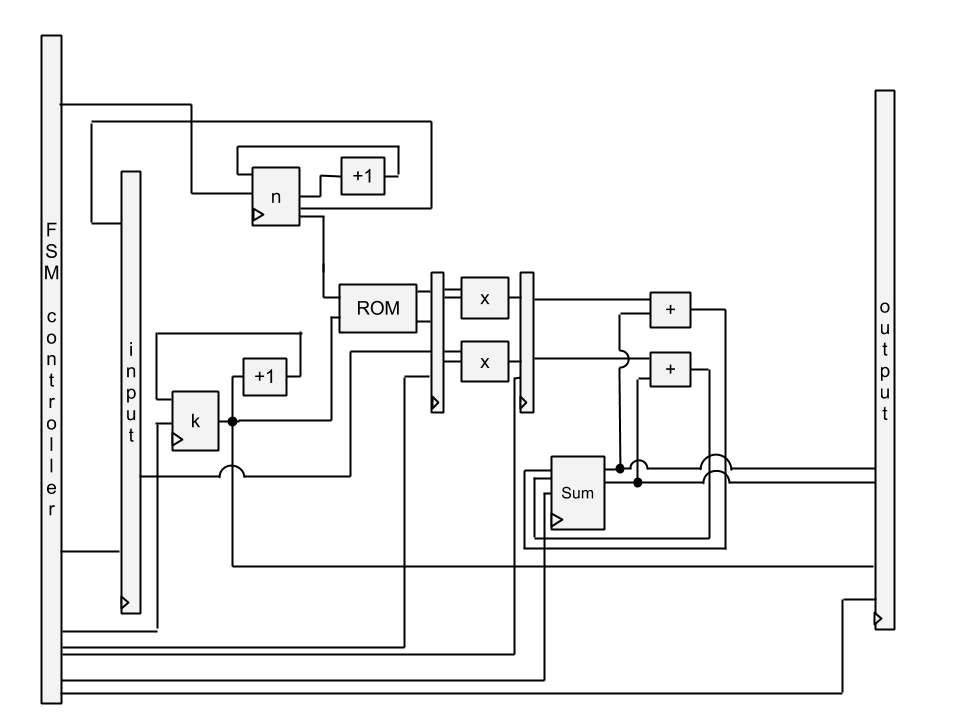
\includegraphics[width=4in]{dft-unit}
\end{frame}

\begin{frame}{Recombination Unit}
	\centering
	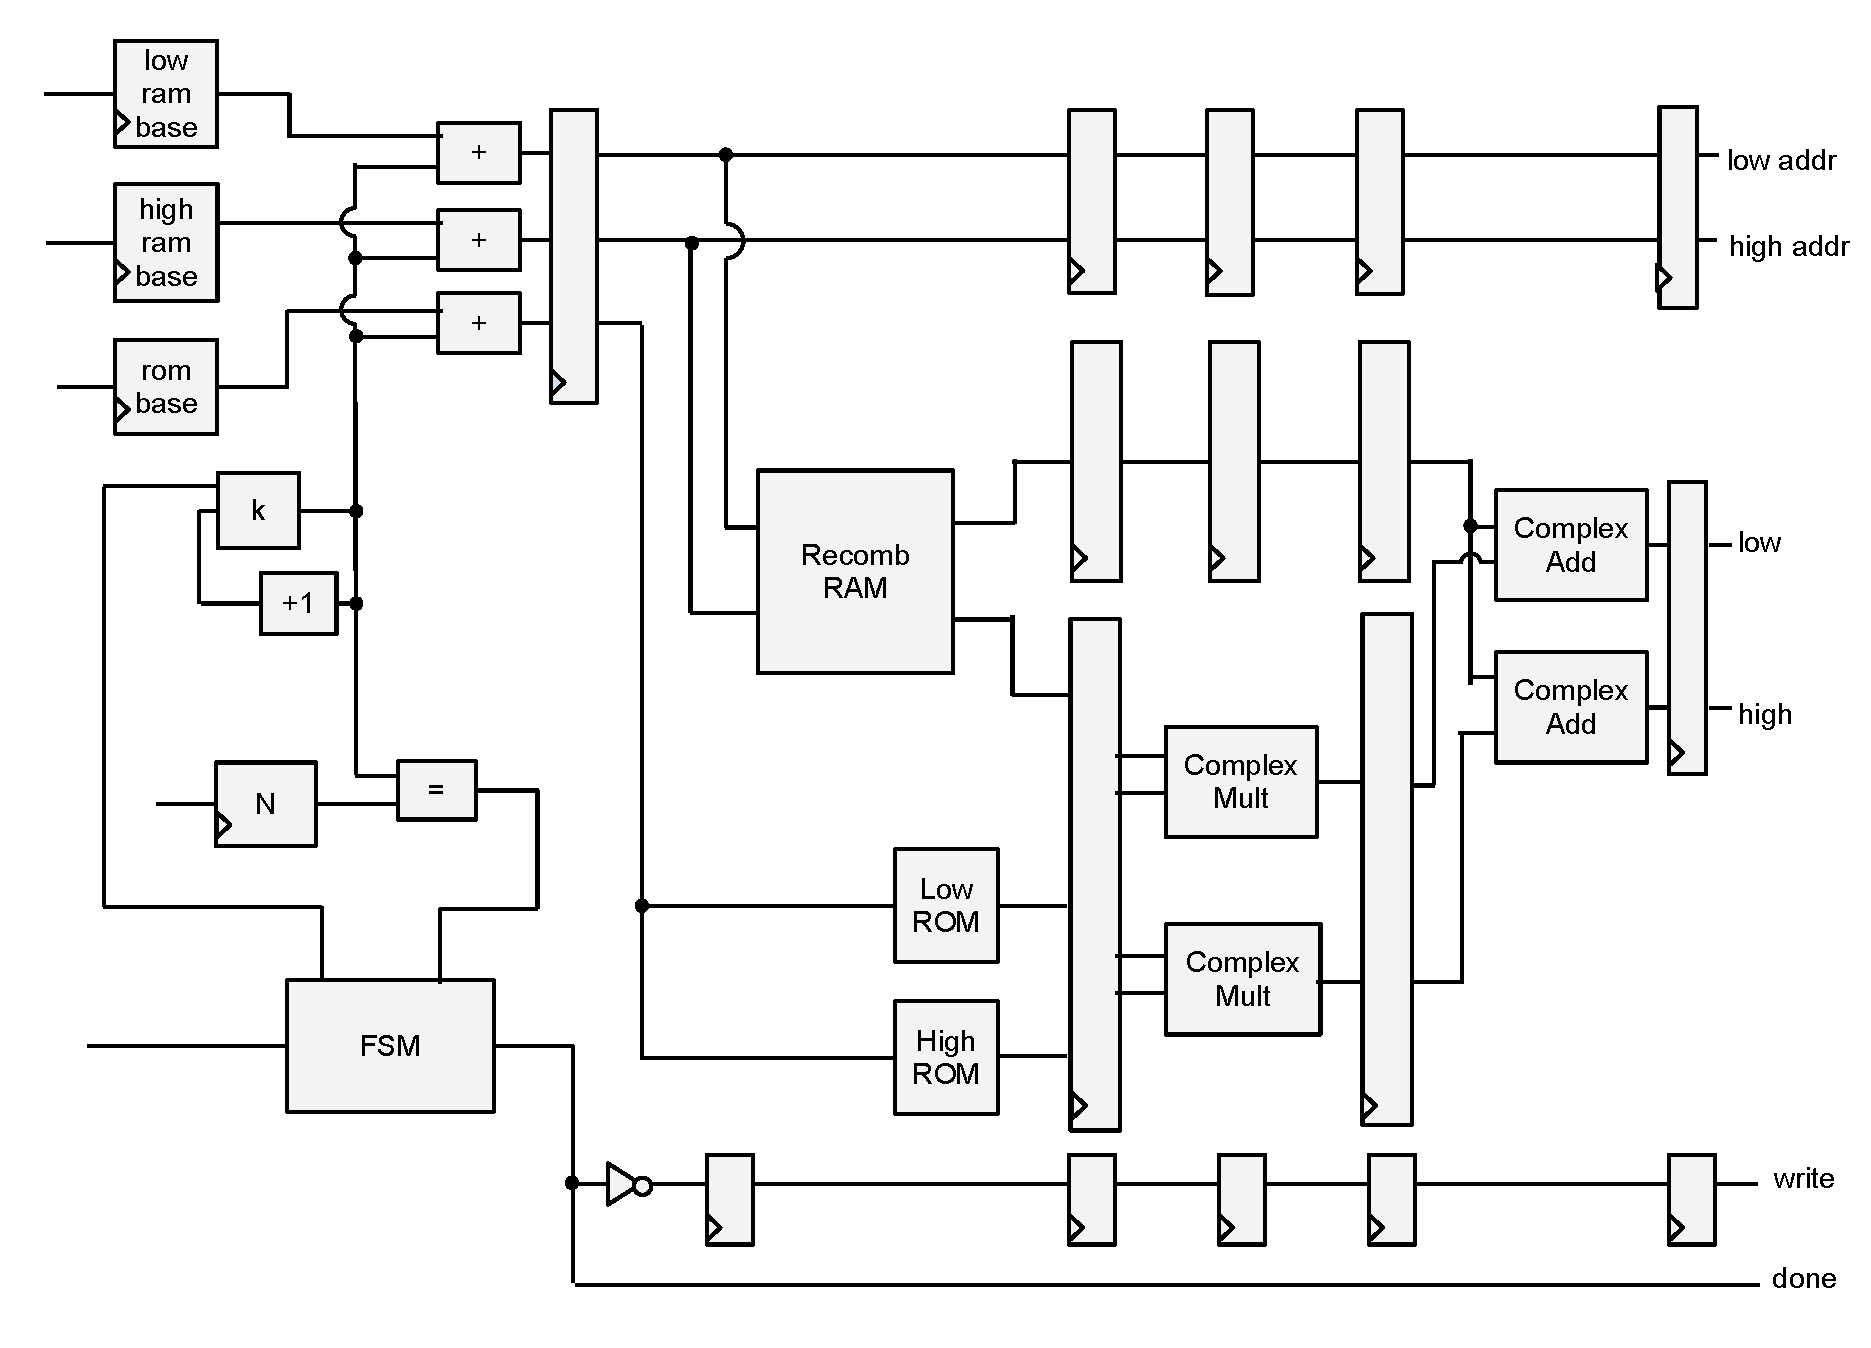
\includegraphics[width=4in]{recombinator}
\end{frame}

\begin{frame}{Complex Multiplier}
	\centering
	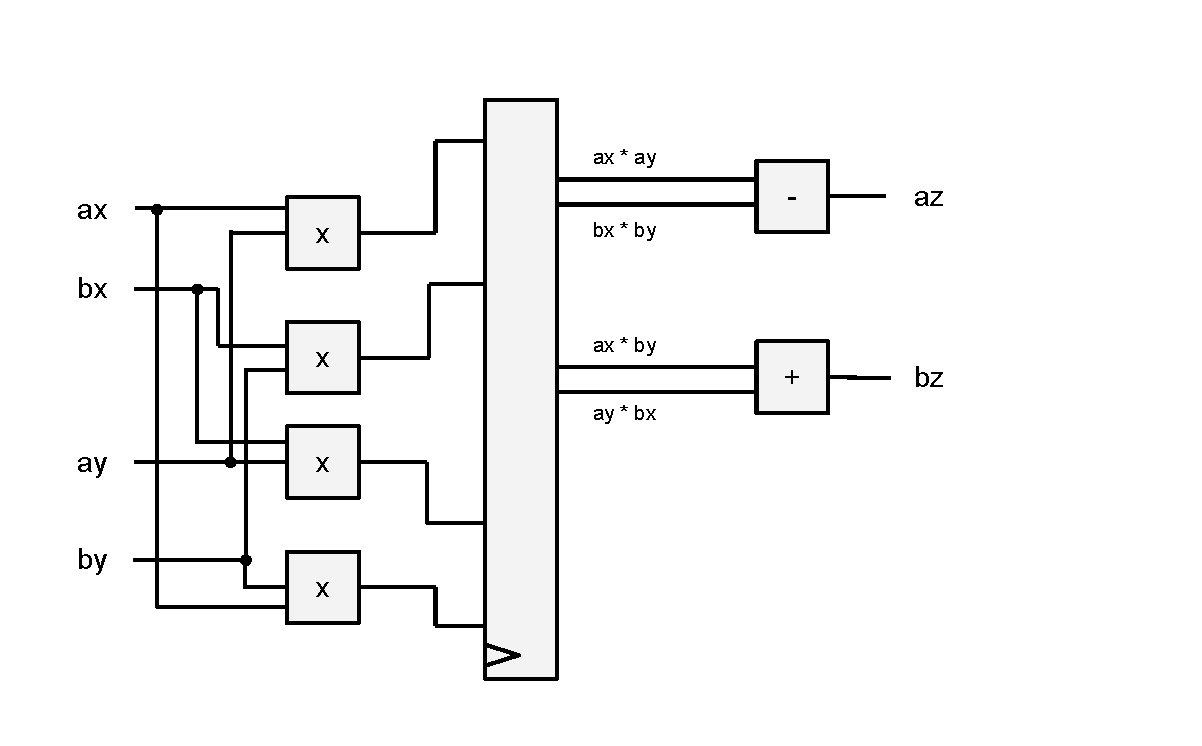
\includegraphics[width=4in]{complex-mult}
\end{frame}

\begin{frame}{Visualizer}
	\centering
	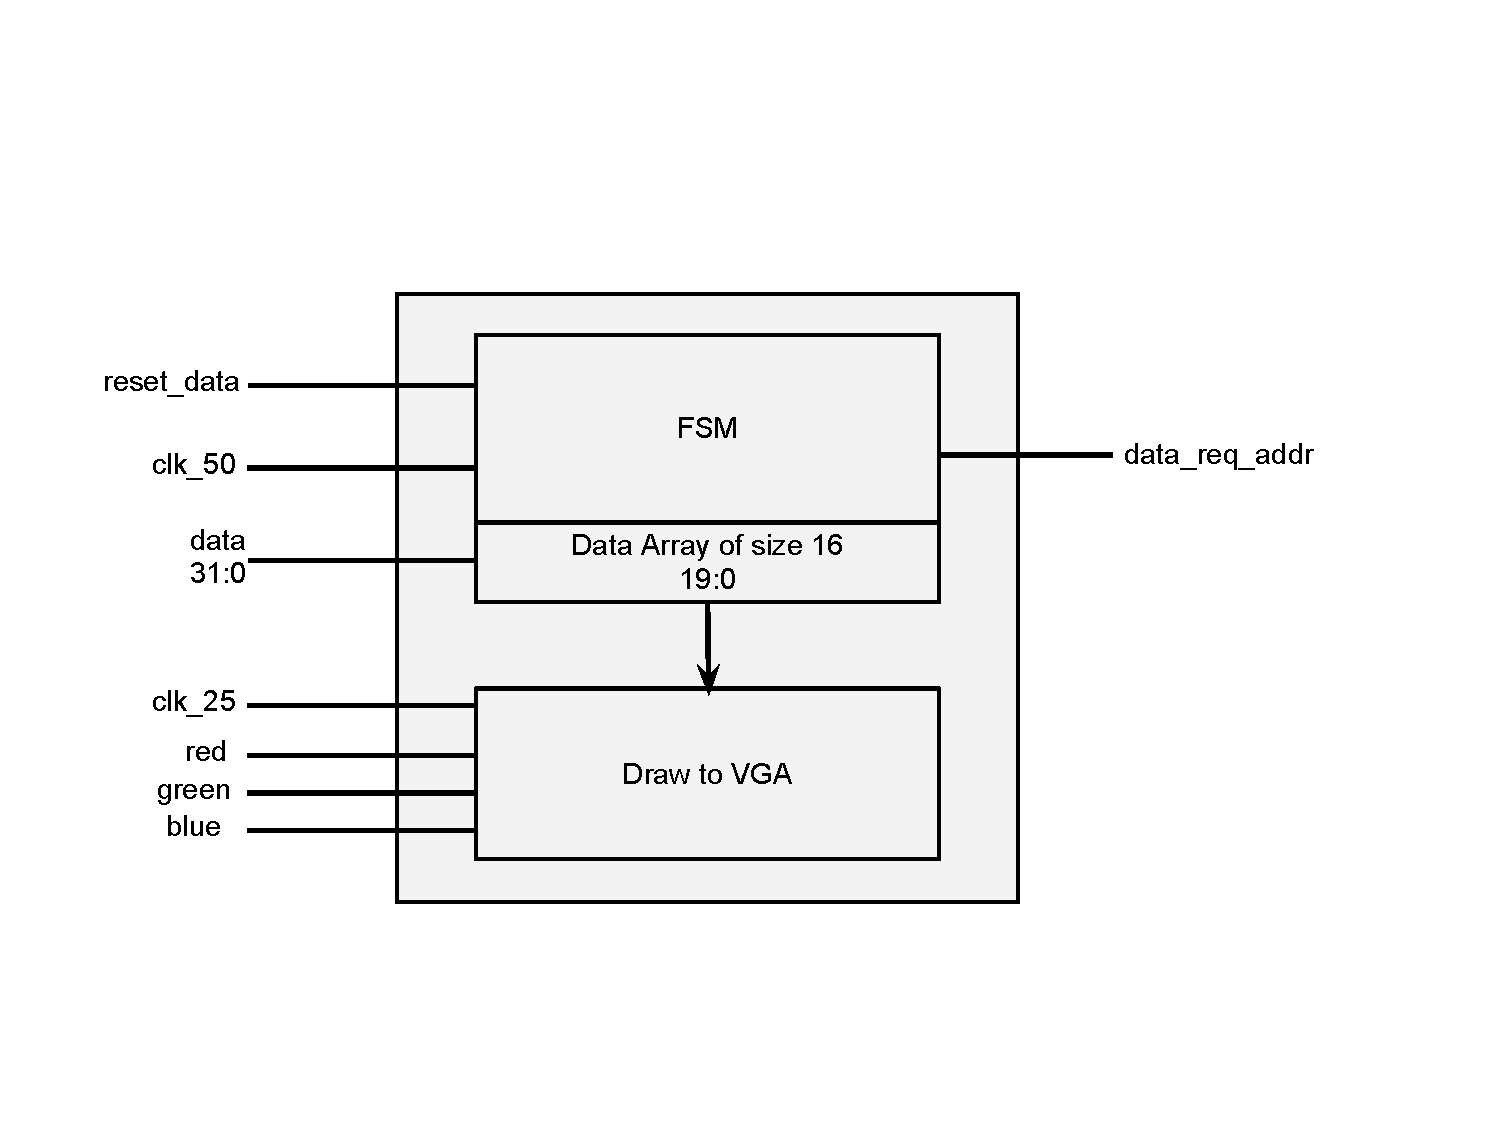
\includegraphics[width=4in]{viz_block_diagram}
\end{frame}

\begin{frame}{Conductor}
	\centering
    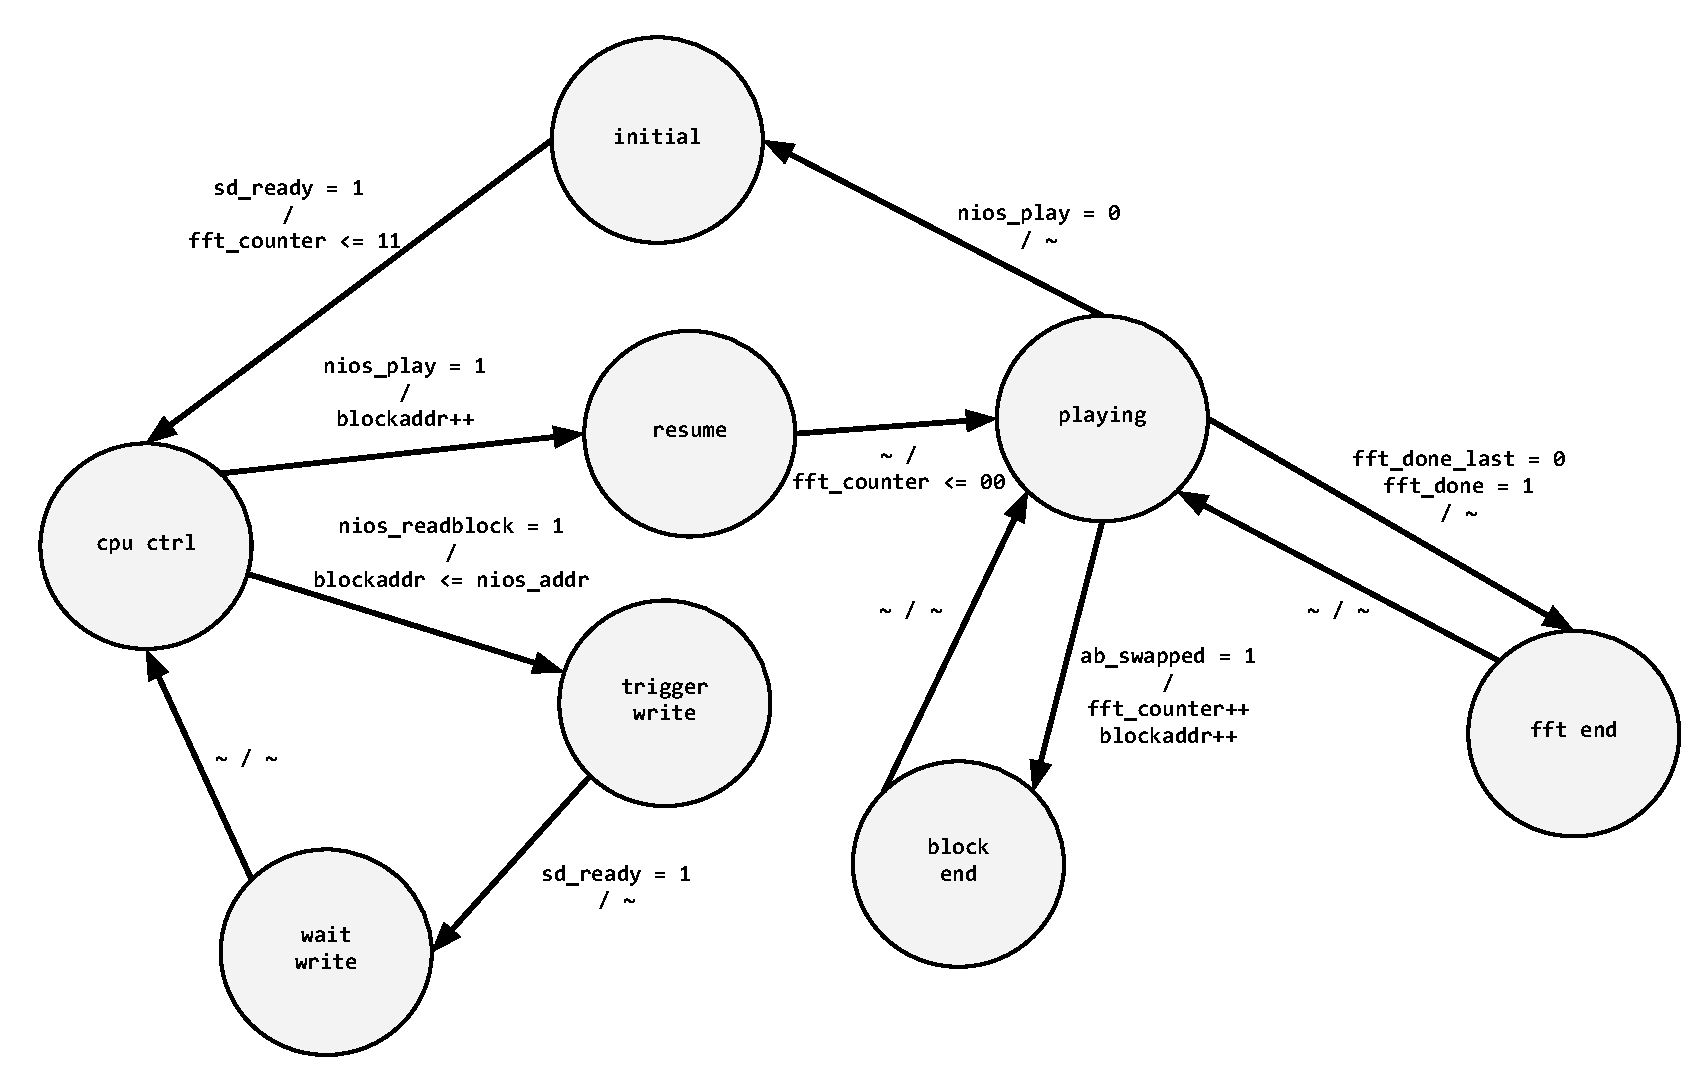
\includegraphics[width=4in]{conductor_state}
\end{frame}

\end{document}
